\documentclass{article}
\usepackage{amsmath}
\usepackage{tikz}

\begin{document}

\begin{center}
    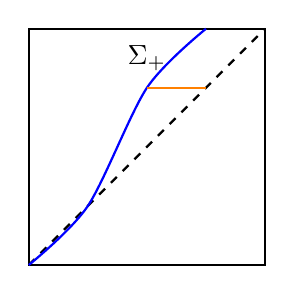
\begin{tikzpicture}[scale=1.5]
        % Draw the square
        \draw[thick] (0,0) rectangle (2,2);
        
        % Draw the diagonal line
        \draw[dashed, thick] (0,0) -- (2,2);
        
        % Draw the curve
        \draw[blue, thick] plot [smooth] coordinates {(0,0) (0.5,0.5) (1,1.5) (1.5,2)};
        
        % Draw the horizontal line segment
        \draw[orange, thick] (1,1.5) -- (1.5,1.5);
        
        % Label the set
        \node at (1,1.75) {$\Sigma_+$};
    \end{tikzpicture}
    
    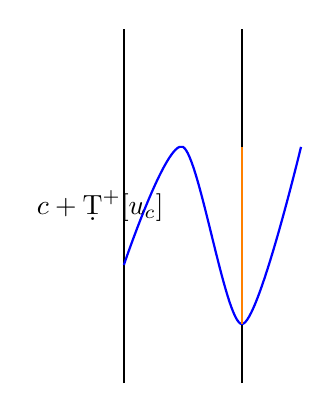
\begin{tikzpicture}[scale=1.5]
        % Draw the vertical lines
        \draw[thick] (0,0) -- (0,3);
        \draw[thick] (1,0) -- (1,3);
        
        % Draw the curve
        \draw[blue, thick] plot [smooth] coordinates {(0,1) (0.5,2) (1,0.5) (1.5,2)};
        
        % Draw the orange line segment
        \draw[orange, thick] (1,0.5) -- (1,2);
        
        % Label the expression
        \node at (-0.2, 1.5) {$c + \d T^+[u_c]$};
    \end{tikzpicture}
    
    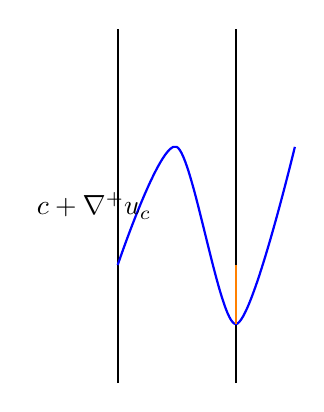
\begin{tikzpicture}[scale=1.5]
        % Draw the vertical lines
        \draw[thick] (0,0) -- (0,3);
        \draw[thick] (1,0) -- (1,3);
        
        % Draw the curve
        \draw[blue, thick] plot [smooth] coordinates {(0,1) (0.5,2) (1,0.5) (1.5,2)};
        
        % Draw the orange line segment
        \draw[orange, thick] (1,0.5) -- (1,1);
        
        % Label the expression
        \node at (-0.2, 1.5) {$c + \nabla^+ u_c$};
    \end{tikzpicture}
\end{center}

\captionof{figure}{The graphs $\operatorname{Graph}(\Sigma_+), \operatorname{Graph}(c+\d T^+[u_c])$ and $\operatorname{Graph}(c+\nabla^+u_c)$ at cohomology class $c=0$ in the pendulum case.}

\end{document}